\documentclass[1p]{elsarticle_modified}
%\bibliographystyle{elsarticle-num}

%\usepackage[colorlinks]{hyperref}
%\usepackage{abbrmath_seonhwa} %\Abb, \Ascr, \Acal ,\Abf, \Afrak
\usepackage{amsfonts}
\usepackage{amssymb}
\usepackage{amsmath}
\usepackage{amsthm}
\usepackage{scalefnt}
\usepackage{amsbsy}
\usepackage{kotex}
\usepackage{caption}
\usepackage{subfig}
\usepackage{color}
\usepackage{graphicx}
\usepackage{xcolor} %% white, black, red, green, blue, cyan, magenta, yellow
\usepackage{float}
\usepackage{setspace}
\usepackage{hyperref}

\usepackage{tikz}
\usetikzlibrary{arrows}

\usepackage{multirow}
\usepackage{array} % fixed length table
\usepackage{hhline}

%%%%%%%%%%%%%%%%%%%%%
\makeatletter
\renewcommand*\env@matrix[1][\arraystretch]{%
	\edef\arraystretch{#1}%
	\hskip -\arraycolsep
	\let\@ifnextchar\new@ifnextchar
	\array{*\c@MaxMatrixCols c}}
\makeatother %https://tex.stackexchange.com/questions/14071/how-can-i-increase-the-line-spacing-in-a-matrix
%%%%%%%%%%%%%%%

\usepackage[normalem]{ulem}

\newcommand{\msout}[1]{\ifmmode\text{\sout{\ensuremath{#1}}}\else\sout{#1}\fi}
%SOURCE: \msout is \stkout macro in https://tex.stackexchange.com/questions/20609/strikeout-in-math-mode

\newcommand{\cancel}[1]{
	\ifmmode
	{\color{red}\msout{#1}}
	\else
	{\color{red}\sout{#1}}
	\fi
}

\newcommand{\add}[1]{
	{\color{blue}\uwave{#1}}
}

\newcommand{\replace}[2]{
	\ifmmode
	{\color{red}\msout{#1}}{\color{blue}\uwave{#2}}
	\else
	{\color{red}\sout{#1}}{\color{blue}\uwave{#2}}
	\fi
}

\newcommand{\Sol}{\mathcal{S}} %segment
\newcommand{\D}{D} %diagram
\newcommand{\A}{\mathcal{A}} %arc


%%%%%%%%%%%%%%%%%%%%%%%%%%%%%5 test

\def\sl{\operatorname{\textup{SL}}(2,\Cbb)}
\def\psl{\operatorname{\textup{PSL}}(2,\Cbb)}
\def\quan{\mkern 1mu \triangleright \mkern 1mu}

\theoremstyle{definition}
\newtheorem{thm}{Theorem}[section]
\newtheorem{prop}[thm]{Proposition}
\newtheorem{lem}[thm]{Lemma}
\newtheorem{ques}[thm]{Question}
\newtheorem{cor}[thm]{Corollary}
\newtheorem{defn}[thm]{Definition}
\newtheorem{exam}[thm]{Example}
\newtheorem{rmk}[thm]{Remark}
\newtheorem{alg}[thm]{Algorithm}

\newcommand{\I}{\sqrt{-1}}
\begin{document}

%\begin{frontmatter}
%
%\title{Boundary parabolic representations of knots up to 8 crossings}
%
%%% Group authors per affiliation:
%\author{Yunhi Cho} 
%\address{Department of Mathematics, University of Seoul, Seoul, Korea}
%\ead{yhcho@uos.ac.kr}
%
%
%\author{Seonhwa Kim} %\fnref{s_kim}}
%\address{Center for Geometry and Physics, Institute for Basic Science, Pohang, 37673, Korea}
%\ead{ryeona17@ibs.re.kr}
%
%\author{Hyuk Kim}
%\address{Department of Mathematical Sciences, Seoul National University, Seoul 08826, Korea}
%\ead{hyukkim@snu.ac.kr}
%
%\author{Seokbeom Yoon}
%\address{Department of Mathematical Sciences, Seoul National University, Seoul, 08826,  Korea}
%\ead{sbyoon15@snu.ac.kr}
%
%\begin{abstract}
%We find all boundary parabolic representation of knots up to 8 crossings.
%
%\end{abstract}
%\begin{keyword}
%    \MSC[2010] 57M25 
%\end{keyword}
%
%\end{frontmatter}

%\linenumbers
%\tableofcontents
%
\newcommand\colored[1]{\textcolor{white}{\rule[-0.35ex]{0.8em}{1.4ex}}\kern-0.8em\color{red} #1}%
%\newcommand\colored[1]{\textcolor{white}{ #1}\kern-2.17ex	\textcolor{white}{ #1}\kern-1.81ex	\textcolor{white}{ #1}\kern-2.15ex\color{red}#1	}

{\Large $\underline{12a_{0268}~(K12a_{0268})}$}

\setlength{\tabcolsep}{10pt}
\renewcommand{\arraystretch}{1.6}
\vspace{1cm}\begin{tabular}{m{100pt}>{\centering\arraybackslash}m{274pt}}
\multirow{5}{120pt}{
	\centering
	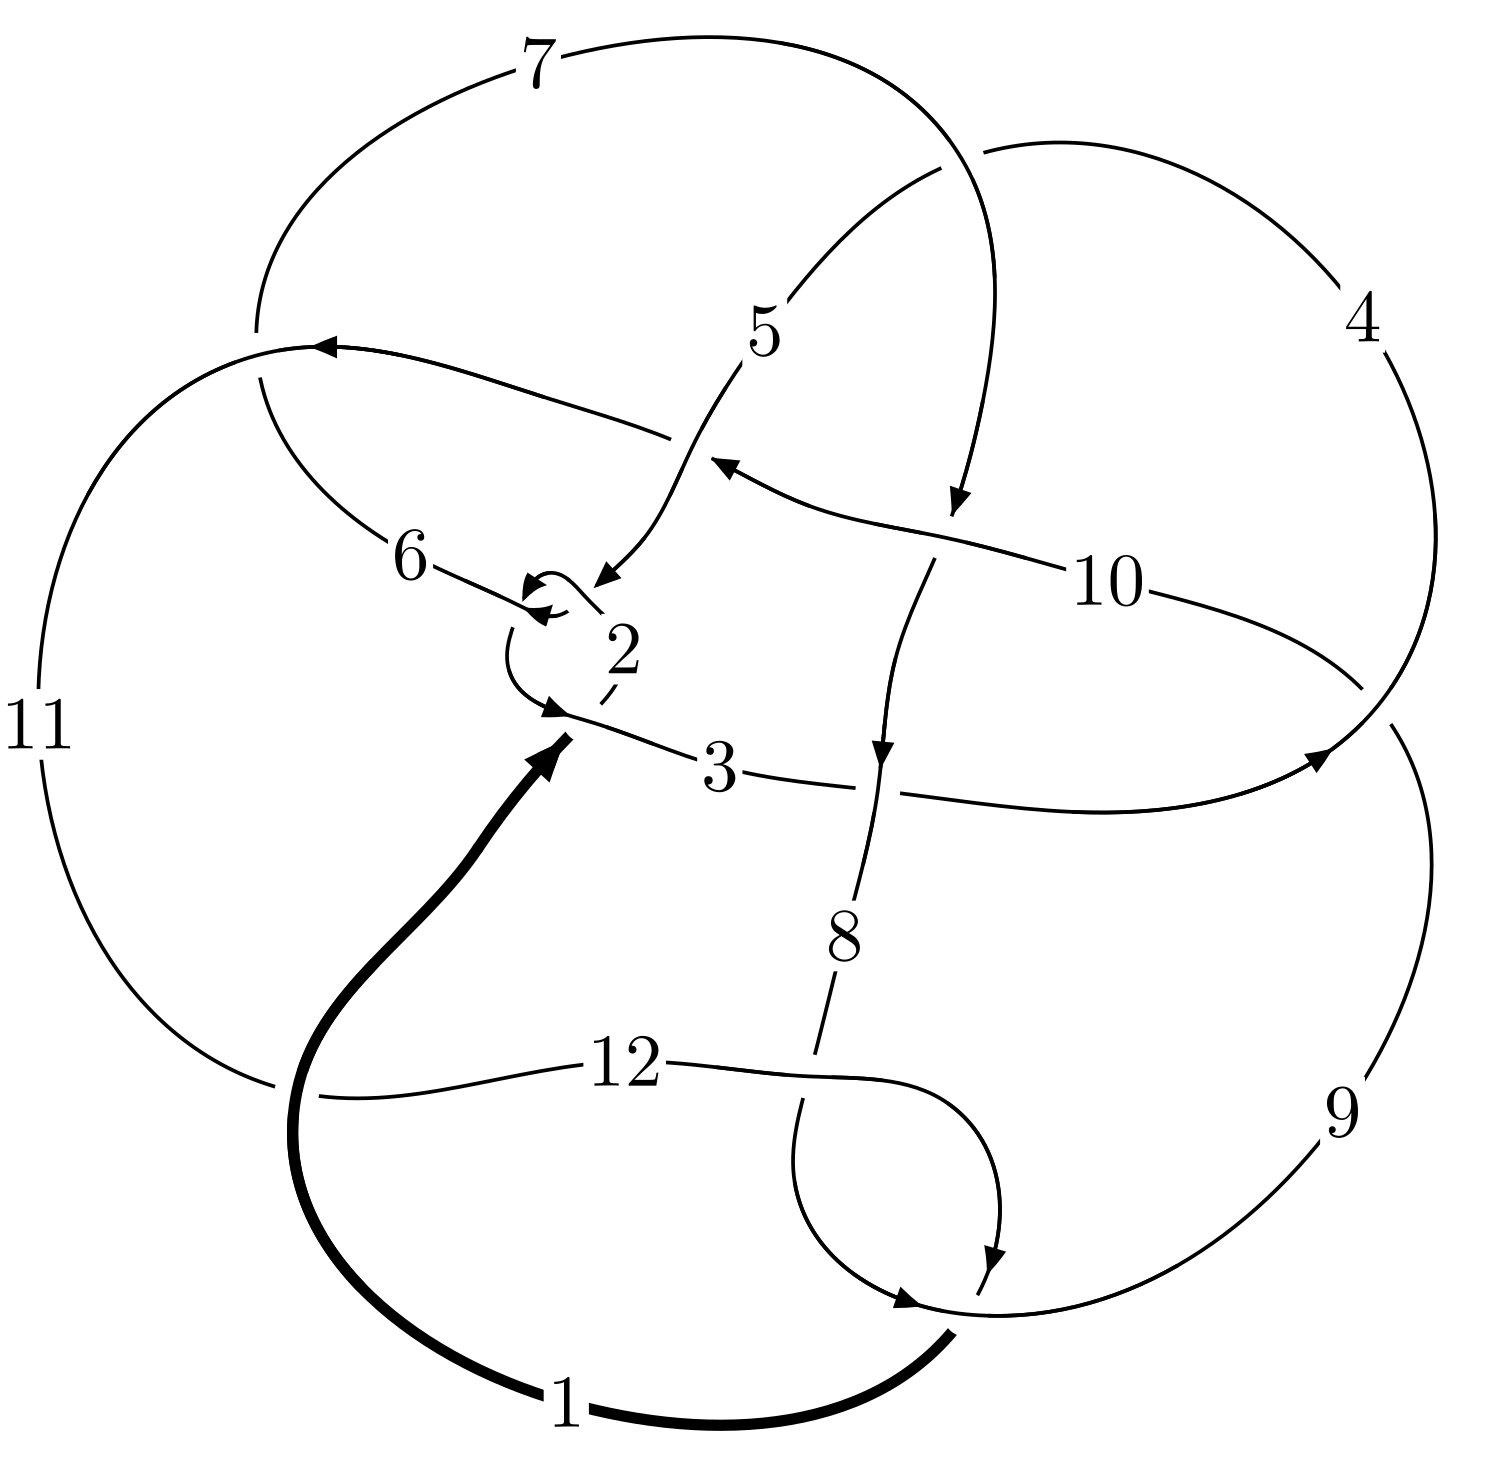
\includegraphics[width=112pt]{../../../GIT/diagram.site/Diagrams/png/1069_12a_0268.png}\\
\ \ \ A knot diagram\footnotemark}&
\allowdisplaybreaks
\textbf{Linearized knot diagam} \\
\cline{2-2}
 &
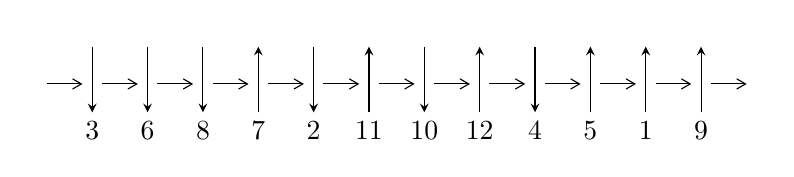
\begin{tikzpicture}[x=20pt, y=17pt]
	% nodes
	\node (C0) at (0, 0) {};
	\node (C1) at (1, 0) {};
	\node (C1U) at (1, +1) {};
	\node (C1D) at (1, -1) {3};

	\node (C2) at (2, 0) {};
	\node (C2U) at (2, +1) {};
	\node (C2D) at (2, -1) {6};

	\node (C3) at (3, 0) {};
	\node (C3U) at (3, +1) {};
	\node (C3D) at (3, -1) {8};

	\node (C4) at (4, 0) {};
	\node (C4U) at (4, +1) {};
	\node (C4D) at (4, -1) {7};

	\node (C5) at (5, 0) {};
	\node (C5U) at (5, +1) {};
	\node (C5D) at (5, -1) {2};

	\node (C6) at (6, 0) {};
	\node (C6U) at (6, +1) {};
	\node (C6D) at (6, -1) {11};

	\node (C7) at (7, 0) {};
	\node (C7U) at (7, +1) {};
	\node (C7D) at (7, -1) {10};

	\node (C8) at (8, 0) {};
	\node (C8U) at (8, +1) {};
	\node (C8D) at (8, -1) {12};

	\node (C9) at (9, 0) {};
	\node (C9U) at (9, +1) {};
	\node (C9D) at (9, -1) {4};

	\node (C10) at (10, 0) {};
	\node (C10U) at (10, +1) {};
	\node (C10D) at (10, -1) {5};

	\node (C11) at (11, 0) {};
	\node (C11U) at (11, +1) {};
	\node (C11D) at (11, -1) {1};

	\node (C12) at (12, 0) {};
	\node (C12U) at (12, +1) {};
	\node (C12D) at (12, -1) {9};
	\node (C13) at (13, 0) {};

	% arrows
	\draw[->,>={angle 60}]
	(C0) edge (C1) (C1) edge (C2) (C2) edge (C3) (C3) edge (C4) (C4) edge (C5) (C5) edge (C6) (C6) edge (C7) (C7) edge (C8) (C8) edge (C9) (C9) edge (C10) (C10) edge (C11) (C11) edge (C12) (C12) edge (C13) ;	\draw[->,>=stealth]
	(C1U) edge (C1D) (C2U) edge (C2D) (C3U) edge (C3D) (C4D) edge (C4U) (C5U) edge (C5D) (C6D) edge (C6U) (C7U) edge (C7D) (C8D) edge (C8U) (C9U) edge (C9D) (C10D) edge (C10U) (C11D) edge (C11U) (C12D) edge (C12U) ;
	\end{tikzpicture} \\
\hhline{~~} \\& 
\textbf{Solving Sequence} \\ \cline{2-2} 
 &
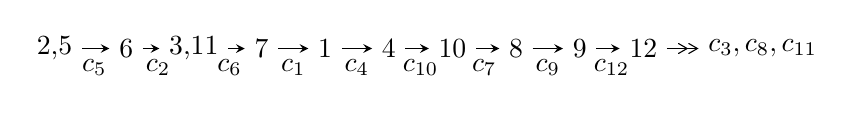
\begin{tikzpicture}[x=23pt, y=7pt]
	% node
	\node (A0) at (-1/8, 0) {2,5};
	\node (A1) at (1, 0) {6};
	\node (A2) at (33/16, 0) {3,11};
	\node (A3) at (25/8, 0) {7};
	\node (A4) at (33/8, 0) {1};
	\node (A5) at (41/8, 0) {4};
	\node (A6) at (49/8, 0) {10};
	\node (A7) at (57/8, 0) {8};
	\node (A8) at (65/8, 0) {9};
	\node (A9) at (73/8, 0) {12};
	\node (C1) at (1/2, -1) {$c_{5}$};
	\node (C2) at (3/2, -1) {$c_{2}$};
	\node (C3) at (21/8, -1) {$c_{6}$};
	\node (C4) at (29/8, -1) {$c_{1}$};
	\node (C5) at (37/8, -1) {$c_{4}$};
	\node (C6) at (45/8, -1) {$c_{10}$};
	\node (C7) at (53/8, -1) {$c_{7}$};
	\node (C8) at (61/8, -1) {$c_{9}$};
	\node (C9) at (69/8, -1) {$c_{12}$};
	\node (A10) at (11, 0) {$c_{3},c_{8},c_{11}$};

	% edge
	\draw[->,>=stealth]	
	(A0) edge (A1) (A1) edge (A2) (A2) edge (A3) (A3) edge (A4) (A4) edge (A5) (A5) edge (A6) (A6) edge (A7) (A7) edge (A8) (A8) edge (A9) ;
	\draw[->>,>={angle 60}]	
	(A9) edge (A10);
\end{tikzpicture} \\ 

\end{tabular} \\

\footnotetext{
The image of knot diagram is generated by the software ``\textbf{Draw programme}" developed by Andrew Bartholomew(\url{http://www.layer8.co.uk/maths/draw/index.htm\#Running-draw}), where we modified some parts for our purpose(\url{https://github.com/CATsTAILs/LinksPainter}).
}\phantom \\ \newline 
\centering \textbf{Ideals for irreducible components\footnotemark of $X_{\text{par}}$} 
 
\begin{align*}
I^u_{1}&=\langle 
6 u^{25}-4 u^{24}+\cdots+b-2,\;-9 u^{25}+23 u^{24}+\cdots+a+31,\;u^{26}-2 u^{25}+\cdots-4 u+1\rangle \\
I^u_{2}&=\langle 
- u^2 a+a u+u^2+b- u+1,\;- u^2 a+a^2+3 a u+u^2-2 a-3 u+2,\;u^3- u^2+1\rangle \\
I^u_{3}&=\langle 
-50 a^5+47 a^4-54 a^3+71 a^2+1503 b-998 a+328,\;a^6+2 a^4+2 a^3+6 a^2+11 a-23,\;u+1\rangle \\
\\
\end{align*}
\raggedright * 3 irreducible components of $\dim_{\mathbb{C}}=0$, with total 38 representations.\\
\footnotetext{All coefficients of polynomials are rational numbers. But the coefficients are sometimes approximated in decimal forms when there is not enough margin.}
\newpage
\renewcommand{\arraystretch}{1}
\centering \section*{I. $I^u_{1}= \langle 6 u^{25}-4 u^{24}+\cdots+b-2,\;-9 u^{25}+23 u^{24}+\cdots+a+31,\;u^{26}-2 u^{25}+\cdots-4 u+1 \rangle$}
\flushleft \textbf{(i) Arc colorings}\\
\begin{tabular}{m{7pt} m{180pt} m{7pt} m{180pt} }
\flushright $a_{2}=$&$\begin{pmatrix}0\\u\end{pmatrix}$ \\
\flushright $a_{5}=$&$\begin{pmatrix}1\\0\end{pmatrix}$ \\
\flushright $a_{6}=$&$\begin{pmatrix}1\\u^2\end{pmatrix}$ \\
\flushright $a_{3}=$&$\begin{pmatrix}- u\\- u^3+u\end{pmatrix}$ \\
\flushright $a_{11}=$&$\begin{pmatrix}9 u^{25}-23 u^{24}+\cdots+69 u-31\\-6 u^{25}+4 u^{24}+\cdots-8 u+2\end{pmatrix}$ \\
\flushright $a_{7}=$&$\begin{pmatrix}-4 u^{25}+14 u^{24}+\cdots-43 u+27\\- u^{25}+u^{24}+\cdots+2 u^2-4 u\end{pmatrix}$ \\
\flushright $a_{1}=$&$\begin{pmatrix}u^3\\u^5- u^3+u\end{pmatrix}$ \\
\flushright $a_{4}=$&$\begin{pmatrix}-32 u^{25}+28 u^{24}+\cdots-79 u+9\\10 u^{25}-11 u^{24}+\cdots+34 u-10\end{pmatrix}$ \\
\flushright $a_{10}=$&$\begin{pmatrix}15 u^{25}-27 u^{24}+\cdots+77 u-33\\-6 u^{25}+4 u^{24}+\cdots-8 u+2\end{pmatrix}$ \\
\flushright $a_{8}=$&$\begin{pmatrix}37 u^{25}-38 u^{24}+\cdots+103 u-23\\-16 u^{25}+5 u^{24}+\cdots-19 u+1\end{pmatrix}$ \\
\flushright $a_{9}=$&$\begin{pmatrix}21 u^{25}-12 u^{24}+\cdots+25 u+4\\-25 u^{25}+29 u^{24}+\cdots-80 u+22\end{pmatrix}$ \\
\flushright $a_{12}=$&$\begin{pmatrix}17 u^{25}-37 u^{24}+\cdots+107 u-43\\-6 u^{25}+12 u^{24}+\cdots-29 u+12\end{pmatrix}$\\&\end{tabular}
\flushleft \textbf{(ii) Obstruction class $= 1$}\\~\\
\flushleft \textbf{(iii) Cusp Shapes $= 61 u^{25}-54 u^{24}-343 u^{23}+372 u^{22}+878 u^{21}-898 u^{20}-1579 u^{19}+1127 u^{18}+2535 u^{17}-859 u^{16}-3329 u^{15}+282 u^{14}+3349 u^{13}+450 u^{12}-2660 u^{11}-969 u^{10}+2067 u^9+348 u^8-518 u^7-770 u^6+524 u^5+209 u^4-85 u^3-178 u^2+111 u-12$}\\~\\
\newpage\renewcommand{\arraystretch}{1}
\flushleft \textbf{(iv) u-Polynomials at the component}\newline \\
\begin{tabular}{m{50pt}|m{274pt}}
Crossings & \hspace{64pt}u-Polynomials at each crossing \\
\hline $$\begin{aligned}c_{1}\end{aligned}$$&$\begin{aligned}
&u^{26}-12 u^{25}+\cdots-6 u+1
\end{aligned}$\\
\hline $$\begin{aligned}c_{2},c_{12}\end{aligned}$$&$\begin{aligned}
&u^{26}+2 u^{25}+\cdots+4 u+1
\end{aligned}$\\
\hline $$\begin{aligned}c_{3}\end{aligned}$$&$\begin{aligned}
&u^{26}+2 u^{25}+\cdots-2 u^2+1
\end{aligned}$\\
\hline $$\begin{aligned}c_{4}\end{aligned}$$&$\begin{aligned}
&u^{26}-3 u^{24}+\cdots+167 u+85
\end{aligned}$\\
\hline $$\begin{aligned}c_{5},c_{8}\end{aligned}$$&$\begin{aligned}
&u^{26}-2 u^{25}+\cdots-4 u+1
\end{aligned}$\\
\hline $$\begin{aligned}c_{6}\end{aligned}$$&$\begin{aligned}
&u^{26}-2 u^{25}+\cdots-2 u^2+1
\end{aligned}$\\
\hline $$\begin{aligned}c_{7}\end{aligned}$$&$\begin{aligned}
&u^{26}-3 u^{24}+\cdots-167 u+85
\end{aligned}$\\
\hline $$\begin{aligned}c_{9}\end{aligned}$$&$\begin{aligned}
&u^{26}+u^{24}+\cdots+u^2+1
\end{aligned}$\\
\hline $$\begin{aligned}c_{10}\end{aligned}$$&$\begin{aligned}
&u^{26}+u^{24}+\cdots+u^2+1
\end{aligned}$\\
\hline $$\begin{aligned}c_{11}\end{aligned}$$&$\begin{aligned}
&u^{26}+12 u^{25}+\cdots+6 u+1
\end{aligned}$\\
\hline
\end{tabular}\\~\\
\newpage\renewcommand{\arraystretch}{1}
\flushleft \textbf{(v) Riley Polynomials at the component}\newline \\
\begin{tabular}{m{50pt}|m{274pt}}
Crossings & \hspace{64pt}Riley Polynomials at each crossing \\
\hline $$\begin{aligned}c_{1},c_{11}\end{aligned}$$&$\begin{aligned}
&y^{26}-8 y^{24}+\cdots+22 y+1
\end{aligned}$\\
\hline $$\begin{aligned}c_{2},c_{5},c_{8}\\c_{12}\end{aligned}$$&$\begin{aligned}
&y^{26}-12 y^{25}+\cdots-6 y+1
\end{aligned}$\\
\hline $$\begin{aligned}c_{3},c_{6}\end{aligned}$$&$\begin{aligned}
&y^{26}-20 y^{25}+\cdots-4 y+1
\end{aligned}$\\
\hline $$\begin{aligned}c_{4},c_{7}\end{aligned}$$&$\begin{aligned}
&y^{26}-6 y^{25}+\cdots+51331 y+7225
\end{aligned}$\\
\hline $$\begin{aligned}c_{9},c_{10}\end{aligned}$$&$\begin{aligned}
&y^{26}+2 y^{25}+\cdots+2 y+1
\end{aligned}$\\
\hline
\end{tabular}\\~\\
\newpage\flushleft \textbf{(vi) Complex Volumes and Cusp Shapes}
$$\begin{array}{c|c|c}  
\text{Solutions to }I^u_{1}& \I (\text{vol} + \sqrt{-1}CS) & \text{Cusp shape}\\
 \hline 
\begin{aligned}
u &= -0.461384 + 0.912562 I \\
a &= -0.080894 - 0.407248 I \\
b &= \phantom{-}0.575155 + 0.340795 I\end{aligned}
 & \phantom{-}1.12657 + 3.32893 I & \phantom{-}5.69551 - 1.13200 I \\ \hline\begin{aligned}
u &= -0.461384 - 0.912562 I \\
a &= -0.080894 + 0.407248 I \\
b &= \phantom{-}0.575155 - 0.340795 I\end{aligned}
 & \phantom{-}1.12657 - 3.32893 I & \phantom{-}5.69551 + 1.13200 I \\ \hline\begin{aligned}
u &= \phantom{-}0.849370 + 0.605420 I \\
a &= -1.25013 - 1.25835 I \\
b &= -0.14769 - 1.58072 I\end{aligned}
 & \phantom{-}3.52283 - 2.38934 I & \phantom{-}15.7660 + 2.5226 I \\ \hline\begin{aligned}
u &= \phantom{-}0.849370 - 0.605420 I \\
a &= -1.25013 + 1.25835 I \\
b &= -0.14769 + 1.58072 I\end{aligned}
 & \phantom{-}3.52283 + 2.38934 I & \phantom{-}15.7660 - 2.5226 I \\ \hline\begin{aligned}
u &= -0.762938 + 0.732586 I \\
a &= -0.154380 + 0.405636 I \\
b &= \phantom{-}0.965729 + 0.259552 I\end{aligned}
 & \phantom{-0.000000 -}5.79972 I & \phantom{-0.000000 } 0. - 8.96426 I \\ \hline\begin{aligned}
u &= -0.762938 - 0.732586 I \\
a &= -0.154380 - 0.405636 I \\
b &= \phantom{-}0.965729 - 0.259552 I\end{aligned}
 & \phantom{-0.000000 } -5.79972 I & \phantom{-0.000000 -}0. + 8.96426 I \\ \hline\begin{aligned}
u &= \phantom{-}0.998814 + 0.491144 I \\
a &= \phantom{-}0.29293 + 2.27648 I \\
b &= -1.11561 + 0.93756 I\end{aligned}
 & -2.06063 - 7.20438 I & -4.87470 + 7.46295 I \\ \hline\begin{aligned}
u &= \phantom{-}0.998814 - 0.491144 I \\
a &= \phantom{-}0.29293 - 2.27648 I \\
b &= -1.11561 - 0.93756 I\end{aligned}
 & -2.06063 + 7.20438 I & -4.87470 - 7.46295 I \\ \hline\begin{aligned}
u &= \phantom{-}0.742293 + 0.445659 I \\
a &= \phantom{-}0.246099 - 0.102462 I \\
b &= \phantom{-}1.28686 + 0.76250 I\end{aligned}
 & -1.12657 + 3.32893 I & -5.69551 - 1.13200 I \\ \hline\begin{aligned}
u &= \phantom{-}0.742293 - 0.445659 I \\
a &= \phantom{-}0.246099 + 0.102462 I \\
b &= \phantom{-}1.28686 - 0.76250 I\end{aligned}
 & -1.12657 - 3.32893 I & -5.69551 + 1.13200 I\\
 \hline 
 \end{array}$$\newpage$$\begin{array}{c|c|c}  
\text{Solutions to }I^u_{1}& \I (\text{vol} + \sqrt{-1}CS) & \text{Cusp shape}\\
 \hline 
\begin{aligned}
u &= -0.316384 + 0.759790 I \\
a &= \phantom{-}0.202465 + 1.071890 I \\
b &= -0.525339 - 0.441494 I\end{aligned}
 & \phantom{-}2.06063 + 7.20438 I & \phantom{-}4.87470 - 7.46295 I \\ \hline\begin{aligned}
u &= -0.316384 - 0.759790 I \\
a &= \phantom{-}0.202465 - 1.071890 I \\
b &= -0.525339 + 0.441494 I\end{aligned}
 & \phantom{-}2.06063 - 7.20438 I & \phantom{-}4.87470 + 7.46295 I \\ \hline\begin{aligned}
u &= \phantom{-}1.081650 + 0.521444 I \\
a &= \phantom{-}0.05036 + 1.94989 I \\
b &= -0.811958 + 0.761507 I\end{aligned}
 & -1.82571 - 6.70629 I & -2.75982 + 7.40474 I \\ \hline\begin{aligned}
u &= \phantom{-}1.081650 - 0.521444 I \\
a &= \phantom{-}0.05036 - 1.94989 I \\
b &= -0.811958 - 0.761507 I\end{aligned}
 & -1.82571 + 6.70629 I & -2.75982 - 7.40474 I \\ \hline\begin{aligned}
u &= \phantom{-}0.516527 + 0.544349 I \\
a &= -0.92356 - 1.49397 I \\
b &= -0.655244 - 0.614530 I\end{aligned}
 & \phantom{-}1.82571 + 6.70629 I & \phantom{-}2.75982 - 7.40474 I \\ \hline\begin{aligned}
u &= \phantom{-}0.516527 - 0.544349 I \\
a &= -0.92356 + 1.49397 I \\
b &= -0.655244 + 0.614530 I\end{aligned}
 & \phantom{-}1.82571 - 6.70629 I & \phantom{-}2.75982 + 7.40474 I \\ \hline\begin{aligned}
u &= \phantom{-}1.089350 + 0.612332 I \\
a &= -0.17797 - 1.62097 I \\
b &= \phantom{-}0.581197 - 0.813763 I\end{aligned}
 & \phantom{-0.000000 } -11.5593 I & \phantom{-0.000000 -}0. + 10.56005 I \\ \hline\begin{aligned}
u &= \phantom{-}1.089350 - 0.612332 I \\
a &= -0.17797 + 1.62097 I \\
b &= \phantom{-}0.581197 + 0.813763 I\end{aligned}
 & \phantom{-0.000000 -}11.5593 I & \phantom{-0.000000 } 0. - 10.56005 I \\ \hline\begin{aligned}
u &= -0.632233 + 0.402098 I \\
a &= \phantom{-}2.06829 - 1.29149 I \\
b &= -0.531949 - 0.961805 I\end{aligned}
 & \phantom{-}2.02248 + 0.44868 I & \phantom{-}1.93644 - 3.28945 I \\ \hline\begin{aligned}
u &= -0.632233 - 0.402098 I \\
a &= \phantom{-}2.06829 + 1.29149 I \\
b &= -0.531949 + 0.961805 I\end{aligned}
 & \phantom{-}2.02248 - 0.44868 I & \phantom{-}1.93644 + 3.28945 I\\
 \hline 
 \end{array}$$\newpage$$\begin{array}{c|c|c}  
\text{Solutions to }I^u_{1}& \I (\text{vol} + \sqrt{-1}CS) & \text{Cusp shape}\\
 \hline 
\begin{aligned}
u &= -1.193370 + 0.413519 I \\
a &= -0.631044 + 0.511481 I \\
b &= -0.440341 + 0.796171 I\end{aligned}
 & -2.02248 - 0.44868 I & -1.93644 + 3.28945 I \\ \hline\begin{aligned}
u &= -1.193370 - 0.413519 I \\
a &= -0.631044 - 0.511481 I \\
b &= -0.440341 - 0.796171 I\end{aligned}
 & -2.02248 + 0.44868 I & -1.93644 - 3.28945 I \\ \hline\begin{aligned}
u &= \phantom{-}0.583202 + 0.387797 I \\
a &= -0.56568 + 1.58491 I \\
b &= \phantom{-}0.877784 + 0.479057 I\end{aligned}
 & \phantom{-0.000000 -}2.72365 I & \phantom{-0.000000 } 0. - 5.95098 I \\ \hline\begin{aligned}
u &= \phantom{-}0.583202 - 0.387797 I \\
a &= -0.56568 - 1.58491 I \\
b &= \phantom{-}0.877784 - 0.479057 I\end{aligned}
 & \phantom{-0.000000 } -2.72365 I & \phantom{-0.000000 -}0. + 5.95098 I \\ \hline\begin{aligned}
u &= -1.49489 + 0.08893 I \\
a &= -0.076473 + 0.557618 I \\
b &= -0.058595 + 0.627148 I\end{aligned}
 & -3.52283 + 2.38934 I & -15.7660 - 2.5226 I \\ \hline\begin{aligned}
u &= -1.49489 - 0.08893 I \\
a &= -0.076473 - 0.557618 I \\
b &= -0.058595 - 0.627148 I\end{aligned}
 & -3.52283 - 2.38934 I & -15.7660 + 2.5226 I\\
 \hline 
 \end{array}$$\newpage\newpage\renewcommand{\arraystretch}{1}
\centering \section*{II. $I^u_{2}= \langle - u^2 a+a u+u^2+b- u+1,\;- u^2 a+a^2+3 a u+u^2-2 a-3 u+2,\;u^3- u^2+1 \rangle$}
\flushleft \textbf{(i) Arc colorings}\\
\begin{tabular}{m{7pt} m{180pt} m{7pt} m{180pt} }
\flushright $a_{2}=$&$\begin{pmatrix}0\\u\end{pmatrix}$ \\
\flushright $a_{5}=$&$\begin{pmatrix}1\\0\end{pmatrix}$ \\
\flushright $a_{6}=$&$\begin{pmatrix}1\\u^2\end{pmatrix}$ \\
\flushright $a_{3}=$&$\begin{pmatrix}- u\\- u^2+u+1\end{pmatrix}$ \\
\flushright $a_{11}=$&$\begin{pmatrix}a\\u^2 a- a u- u^2+u-1\end{pmatrix}$ \\
\flushright $a_{7}=$&$\begin{pmatrix}- u^2 a+a u+2 u^2-2 u+2\\0\end{pmatrix}$ \\
\flushright $a_{1}=$&$\begin{pmatrix}u^2-1\\- u^2\end{pmatrix}$ \\
\flushright $a_{4}=$&$\begin{pmatrix}1\\0\end{pmatrix}$ \\
\flushright $a_{10}=$&$\begin{pmatrix}- u^2 a+a u+u^2+a- u+1\\u^2 a- a u- u^2+u-1\end{pmatrix}$ \\
\flushright $a_{8}=$&$\begin{pmatrix}- u^2+1\\u^2\end{pmatrix}$ \\
\flushright $a_{9}=$&$\begin{pmatrix}a\\u^2 a- a u- u^2+u-1\end{pmatrix}$ \\
\flushright $a_{12}=$&$\begin{pmatrix}u^2+a-1\\u^2 a- a u-2 u^2+u-1\end{pmatrix}$\\&\end{tabular}
\flushleft \textbf{(ii) Obstruction class $= 1$}\\~\\
\flushleft \textbf{(iii) Cusp Shapes $= -10 u^2 a+17 a u+11 u^2-14 a-17 u+18$}\\~\\
\newpage\renewcommand{\arraystretch}{1}
\flushleft \textbf{(iv) u-Polynomials at the component}\newline \\
\begin{tabular}{m{50pt}|m{274pt}}
Crossings & \hspace{64pt}u-Polynomials at each crossing \\
\hline $$\begin{aligned}c_{1},c_{3}\end{aligned}$$&$\begin{aligned}
&(u^3- u^2+2 u-1)^2
\end{aligned}$\\
\hline $$\begin{aligned}c_{2}\end{aligned}$$&$\begin{aligned}
&(u^3+u^2-1)^2
\end{aligned}$\\
\hline $$\begin{aligned}c_{4}\end{aligned}$$&$\begin{aligned}
&u^6
\end{aligned}$\\
\hline $$\begin{aligned}c_{5}\end{aligned}$$&$\begin{aligned}
&(u^3- u^2+1)^2
\end{aligned}$\\
\hline $$\begin{aligned}c_{6},c_{7}\end{aligned}$$&$\begin{aligned}
&u^6+3 u^5+6 u^4+7 u^3+5 u^2+2 u-1
\end{aligned}$\\
\hline $$\begin{aligned}c_{8},c_{11}\end{aligned}$$&$\begin{aligned}
&(u+1)^6
\end{aligned}$\\
\hline $$\begin{aligned}c_{9},c_{10}\end{aligned}$$&$\begin{aligned}
&u^6+2 u^5-2 u^4-3 u^3+2 u^2+2 u-1
\end{aligned}$\\
\hline $$\begin{aligned}c_{12}\end{aligned}$$&$\begin{aligned}
&(u-1)^6
\end{aligned}$\\
\hline
\end{tabular}\\~\\
\newpage\renewcommand{\arraystretch}{1}
\flushleft \textbf{(v) Riley Polynomials at the component}\newline \\
\begin{tabular}{m{50pt}|m{274pt}}
Crossings & \hspace{64pt}Riley Polynomials at each crossing \\
\hline $$\begin{aligned}c_{1},c_{3}\end{aligned}$$&$\begin{aligned}
&(y^3+3 y^2+2 y-1)^2
\end{aligned}$\\
\hline $$\begin{aligned}c_{2},c_{5}\end{aligned}$$&$\begin{aligned}
&(y^3- y^2+2 y-1)^2
\end{aligned}$\\
\hline $$\begin{aligned}c_{4}\end{aligned}$$&$\begin{aligned}
&y^6
\end{aligned}$\\
\hline $$\begin{aligned}c_{6},c_{7}\end{aligned}$$&$\begin{aligned}
&y^6+3 y^5+4 y^4-3 y^3-15 y^2-14 y+1
\end{aligned}$\\
\hline $$\begin{aligned}c_{8},c_{11},c_{12}\end{aligned}$$&$\begin{aligned}
&(y-1)^6
\end{aligned}$\\
\hline $$\begin{aligned}c_{9},c_{10}\end{aligned}$$&$\begin{aligned}
&y^6-8 y^5+20 y^4-27 y^3+20 y^2-8 y+1
\end{aligned}$\\
\hline
\end{tabular}\\~\\
\newpage\flushleft \textbf{(vi) Complex Volumes and Cusp Shapes}
$$\begin{array}{c|c|c}  
\text{Solutions to }I^u_{2}& \I (\text{vol} + \sqrt{-1}CS) & \text{Cusp shape}\\
 \hline 
\begin{aligned}
u &= \phantom{-}0.877439 + 0.744862 I \\
a &= \phantom{-}0.626026 + 0.207777 I \\
b &= -0.869124 - 0.347901 I\end{aligned}
 & \phantom{-}4.66906 - 2.82812 I & \phantom{-}4.76162 + 1.20354 I \\ \hline\begin{aligned}
u &= \phantom{-}0.877439 + 0.744862 I \\
a &= -1.04326 - 1.13522 I \\
b &= \phantom{-}0.991685 - 0.396961 I\end{aligned}
 & \phantom{-}4.66906 - 2.82812 I & \phantom{-}6.27312 + 3.54360 I \\ \hline\begin{aligned}
u &= \phantom{-}0.877439 - 0.744862 I \\
a &= \phantom{-}0.626026 - 0.207777 I \\
b &= -0.869124 + 0.347901 I\end{aligned}
 & \phantom{-}4.66906 + 2.82812 I & \phantom{-}4.76162 - 1.20354 I \\ \hline\begin{aligned}
u &= \phantom{-}0.877439 - 0.744862 I \\
a &= -1.04326 + 1.13522 I \\
b &= \phantom{-}0.991685 + 0.396961 I\end{aligned}
 & \phantom{-}4.66906 + 2.82812 I & \phantom{-}6.27312 - 3.54360 I \\ \hline\begin{aligned}
u &= -0.754878\phantom{ +0.000000I} \\
a &= \phantom{-}1.41297\phantom{ +0.000000I} \\
b &= -0.452937\phantom{ +0.000000I}\end{aligned}
 & \phantom{-}0.531480\phantom{ +0.000000I} & -8.86450\phantom{ +0.000000I} \\ \hline\begin{aligned}
u &= -0.754878\phantom{ +0.000000I} \\
a &= \phantom{-}3.42151\phantom{ +0.000000I} \\
b &= \phantom{-}2.20781\phantom{ +0.000000I}\end{aligned}
 & \phantom{-}0.531480\phantom{ +0.000000I} & -74.2050\phantom{ +0.000000I}\\
 \hline 
 \end{array}$$\newpage\newpage\renewcommand{\arraystretch}{1}
\centering \section*{III. $I^u_{3}= \langle -50 a^5+1503 b+\cdots-998 a+328,\;a^6+2 a^4+2 a^3+6 a^2+11 a-23,\;u+1 \rangle$}
\flushleft \textbf{(i) Arc colorings}\\
\begin{tabular}{m{7pt} m{180pt} m{7pt} m{180pt} }
\flushright $a_{2}=$&$\begin{pmatrix}0\\-1\end{pmatrix}$ \\
\flushright $a_{5}=$&$\begin{pmatrix}1\\0\end{pmatrix}$ \\
\flushright $a_{6}=$&$\begin{pmatrix}1\\1\end{pmatrix}$ \\
\flushright $a_{3}=$&$\begin{pmatrix}1\\0\end{pmatrix}$ \\
\flushright $a_{11}=$&$\begin{pmatrix}a\\0.0332668 a^{5}-0.0312708 a^{4}+\cdots+0.664005 a-0.218230\end{pmatrix}$ \\
\flushright $a_{7}=$&$\begin{pmatrix}0.0312708 a^{5}+0.0306055 a^{4}+\cdots+0.584165 a+0.234864\\0.0232868 a^{5}-0.0552229 a^{4}+\cdots+0.264804 a+0.713906\end{pmatrix}$ \\
\flushright $a_{1}=$&$\begin{pmatrix}-1\\-1\end{pmatrix}$ \\
\flushright $a_{4}=$&$\begin{pmatrix}0.0372588 a^{5}+0.178310 a^{4}+\cdots+0.823686 a+1.20892\\0.0312708 a^{5}+0.0306055 a^{4}+\cdots+0.584165 a+0.234864\end{pmatrix}$ \\
\flushright $a_{10}=$&$\begin{pmatrix}-0.0332668 a^{5}+0.0312708 a^{4}+\cdots+0.335995 a+0.218230\\0.0332668 a^{5}-0.0312708 a^{4}+\cdots+0.664005 a-0.218230\end{pmatrix}$ \\
\flushright $a_{8}=$&$\begin{pmatrix}0.0312708 a^{5}+0.0306055 a^{4}+\cdots+0.584165 a+0.234864\\0.0232868 a^{5}-0.0552229 a^{4}+\cdots+0.264804 a+0.713906\end{pmatrix}$ \\
\flushright $a_{9}=$&$\begin{pmatrix}0.0525615 a^{5}+0.0372588 a^{4}+\cdots+0.769128 a+0.401863\\0.0113107 a^{5}-0.0172987 a^{4}+\cdots+0.785762 a+0.0991351\end{pmatrix}$ \\
\flushright $a_{12}=$&$\begin{pmatrix}0.0332668 a^{5}-0.0312708 a^{4}+\cdots+0.664005 a-0.218230\\0.0665336 a^{5}-0.0625416 a^{4}+\cdots+0.328011 a-0.436460\end{pmatrix}$\\&\end{tabular}
\flushleft \textbf{(ii) Obstruction class $= 1$}\\~\\
\flushleft \textbf{(iii) Cusp Shapes $= -\frac{625}{1503} a^5+\frac{2341}{1503} a^4-\frac{1394}{501} a^3+\frac{9655}{1503} a^2-\frac{13978}{1503} a+\frac{20132}{1503}$}\\~\\
\newpage\renewcommand{\arraystretch}{1}
\flushleft \textbf{(iv) u-Polynomials at the component}\newline \\
\begin{tabular}{m{50pt}|m{274pt}}
Crossings & \hspace{64pt}u-Polynomials at each crossing \\
\hline $$\begin{aligned}c_{1},c_{2}\end{aligned}$$&$\begin{aligned}
&(u-1)^6
\end{aligned}$\\
\hline $$\begin{aligned}c_{3},c_{4}\end{aligned}$$&$\begin{aligned}
&u^6-3 u^5+6 u^4-7 u^3+5 u^2-2 u-1
\end{aligned}$\\
\hline $$\begin{aligned}c_{5}\end{aligned}$$&$\begin{aligned}
&(u+1)^6
\end{aligned}$\\
\hline $$\begin{aligned}c_{6},c_{11}\end{aligned}$$&$\begin{aligned}
&(u^3+u^2+2 u+1)^2
\end{aligned}$\\
\hline $$\begin{aligned}c_{7}\end{aligned}$$&$\begin{aligned}
&u^6
\end{aligned}$\\
\hline $$\begin{aligned}c_{8}\end{aligned}$$&$\begin{aligned}
&(u^3- u^2+1)^2
\end{aligned}$\\
\hline $$\begin{aligned}c_{9},c_{10}\end{aligned}$$&$\begin{aligned}
&u^6-2 u^5-2 u^4+3 u^3+2 u^2-2 u-1
\end{aligned}$\\
\hline $$\begin{aligned}c_{12}\end{aligned}$$&$\begin{aligned}
&(u^3+u^2-1)^2
\end{aligned}$\\
\hline
\end{tabular}\\~\\
\newpage\renewcommand{\arraystretch}{1}
\flushleft \textbf{(v) Riley Polynomials at the component}\newline \\
\begin{tabular}{m{50pt}|m{274pt}}
Crossings & \hspace{64pt}Riley Polynomials at each crossing \\
\hline $$\begin{aligned}c_{1},c_{2},c_{5}\end{aligned}$$&$\begin{aligned}
&(y-1)^6
\end{aligned}$\\
\hline $$\begin{aligned}c_{3},c_{4}\end{aligned}$$&$\begin{aligned}
&y^6+3 y^5+4 y^4-3 y^3-15 y^2-14 y+1
\end{aligned}$\\
\hline $$\begin{aligned}c_{6},c_{11}\end{aligned}$$&$\begin{aligned}
&(y^3+3 y^2+2 y-1)^2
\end{aligned}$\\
\hline $$\begin{aligned}c_{7}\end{aligned}$$&$\begin{aligned}
&y^6
\end{aligned}$\\
\hline $$\begin{aligned}c_{8},c_{12}\end{aligned}$$&$\begin{aligned}
&(y^3- y^2+2 y-1)^2
\end{aligned}$\\
\hline $$\begin{aligned}c_{9},c_{10}\end{aligned}$$&$\begin{aligned}
&y^6-8 y^5+20 y^4-27 y^3+20 y^2-8 y+1
\end{aligned}$\\
\hline
\end{tabular}\\~\\
\newpage\flushleft \textbf{(vi) Complex Volumes and Cusp Shapes}
$$\begin{array}{c|c|c}  
\text{Solutions to }I^u_{3}& \I (\text{vol} + \sqrt{-1}CS) & \text{Cusp shape}\\
 \hline 
\begin{aligned}
u &= -1.00000\phantom{ +0.000000I} \\
a &= \phantom{-}1.02278\phantom{ +0.000000I} \\
b &= \phantom{-}0.452937\phantom{ +0.000000I}\end{aligned}
 & -0.531480\phantom{ +0.000000I} & \phantom{-}8.86450\phantom{ +0.000000I} \\ \hline\begin{aligned}
u &= -1.00000\phantom{ +0.000000I} \\
a &= -1.63797\phantom{ +0.000000I} \\
b &= -2.20781\phantom{ +0.000000I}\end{aligned}
 & -0.531480\phantom{ +0.000000I} & \phantom{-}74.2050\phantom{ +0.000000I} \\ \hline\begin{aligned}
u &= -1.00000\phantom{ +0.000000I} \\
a &= -0.77661 + 1.70410 I \\
b &= -0.991685 + 0.396961 I\end{aligned}
 & -4.66906 + 2.82812 I & -6.27312 - 3.54360 I \\ \hline\begin{aligned}
u &= -1.00000\phantom{ +0.000000I} \\
a &= -0.77661 - 1.70410 I \\
b &= -0.991685 - 0.396961 I\end{aligned}
 & -4.66906 - 2.82812 I & -6.27312 + 3.54360 I \\ \hline\begin{aligned}
u &= -1.00000\phantom{ +0.000000I} \\
a &= \phantom{-}1.08420 + 1.65504 I \\
b &= \phantom{-}0.869124 + 0.347901 I\end{aligned}
 & -4.66906 + 2.82812 I & -4.76162 - 1.20354 I \\ \hline\begin{aligned}
u &= -1.00000\phantom{ +0.000000I} \\
a &= \phantom{-}1.08420 - 1.65504 I \\
b &= \phantom{-}0.869124 - 0.347901 I\end{aligned}
 & -4.66906 - 2.82812 I & -4.76162 + 1.20354 I\\
 \hline 
 \end{array}$$\newpage
\newpage\renewcommand{\arraystretch}{1}
\centering \section*{ IV. u-Polynomials}
\begin{tabular}{m{50pt}|m{274pt}}
Crossings & \hspace{64pt}u-Polynomials at each crossing \\
\hline $$\begin{aligned}c_{1}\end{aligned}$$&$\begin{aligned}
&((u-1)^6)(u^3- u^2+2 u-1)^2(u^{26}-12 u^{25}+\cdots-6 u+1)
\end{aligned}$\\
\hline $$\begin{aligned}c_{2},c_{12}\end{aligned}$$&$\begin{aligned}
&((u-1)^6)(u^3+u^2-1)^2(u^{26}+2 u^{25}+\cdots+4 u+1)
\end{aligned}$\\
\hline $$\begin{aligned}c_{3}\end{aligned}$$&$\begin{aligned}
&(u^3- u^2+2 u-1)^2(u^6-3 u^5+6 u^4-7 u^3+5 u^2-2 u-1)\\
&\cdot(u^{26}+2 u^{25}+\cdots-2 u^2+1)
\end{aligned}$\\
\hline $$\begin{aligned}c_{4}\end{aligned}$$&$\begin{aligned}
&u^6(u^6-3 u^5+\cdots-2 u-1)(u^{26}-3 u^{24}+\cdots+167 u+85)
\end{aligned}$\\
\hline $$\begin{aligned}c_{5},c_{8}\end{aligned}$$&$\begin{aligned}
&((u+1)^6)(u^3- u^2+1)^2(u^{26}-2 u^{25}+\cdots-4 u+1)
\end{aligned}$\\
\hline $$\begin{aligned}c_{6}\end{aligned}$$&$\begin{aligned}
&(u^3+u^2+2 u+1)^2(u^6+3 u^5+6 u^4+7 u^3+5 u^2+2 u-1)\\
&\cdot(u^{26}-2 u^{25}+\cdots-2 u^2+1)
\end{aligned}$\\
\hline $$\begin{aligned}c_{7}\end{aligned}$$&$\begin{aligned}
&u^6(u^6+3 u^5+\cdots+2 u-1)(u^{26}-3 u^{24}+\cdots-167 u+85)
\end{aligned}$\\
\hline $$\begin{aligned}c_{9}\end{aligned}$$&$\begin{aligned}
&(u^6-2 u^5-2 u^4+3 u^3+2 u^2-2 u-1)\\
&\cdot(u^6+2 u^5+\cdots+2 u-1)(u^{26}+u^{24}+\cdots+u^2+1)
\end{aligned}$\\
\hline $$\begin{aligned}c_{10}\end{aligned}$$&$\begin{aligned}
&(u^6-2 u^5-2 u^4+3 u^3+2 u^2-2 u-1)\\
&\cdot(u^6+2 u^5+\cdots+2 u-1)(u^{26}+u^{24}+\cdots+u^2+1)
\end{aligned}$\\
\hline $$\begin{aligned}c_{11}\end{aligned}$$&$\begin{aligned}
&((u+1)^6)(u^3+u^2+2 u+1)^2(u^{26}+12 u^{25}+\cdots+6 u+1)
\end{aligned}$\\
\hline
\end{tabular}\newpage\renewcommand{\arraystretch}{1}
\centering \section*{ V. Riley Polynomials}
\begin{tabular}{m{50pt}|m{274pt}}
Crossings & \hspace{64pt}Riley Polynomials at each crossing \\
\hline $$\begin{aligned}c_{1},c_{11}\end{aligned}$$&$\begin{aligned}
&((y-1)^6)(y^3+3 y^2+2 y-1)^2(y^{26}-8 y^{24}+\cdots+22 y+1)
\end{aligned}$\\
\hline $$\begin{aligned}c_{2},c_{5},c_{8}\\c_{12}\end{aligned}$$&$\begin{aligned}
&((y-1)^6)(y^3- y^2+2 y-1)^2(y^{26}-12 y^{25}+\cdots-6 y+1)
\end{aligned}$\\
\hline $$\begin{aligned}c_{3},c_{6}\end{aligned}$$&$\begin{aligned}
&(y^3+3 y^2+2 y-1)^2(y^6+3 y^5+4 y^4-3 y^3-15 y^2-14 y+1)\\
&\cdot(y^{26}-20 y^{25}+\cdots-4 y+1)
\end{aligned}$\\
\hline $$\begin{aligned}c_{4},c_{7}\end{aligned}$$&$\begin{aligned}
&y^6(y^6+3 y^5+4 y^4-3 y^3-15 y^2-14 y+1)\\
&\cdot(y^{26}-6 y^{25}+\cdots+51331 y+7225)
\end{aligned}$\\
\hline $$\begin{aligned}c_{9},c_{10}\end{aligned}$$&$\begin{aligned}
&((y^6-8 y^5+\cdots-8 y+1)^{2})(y^{26}+2 y^{25}+\cdots+2 y+1)
\end{aligned}$\\
\hline
\end{tabular}
\vskip 2pc
\end{document}